\addcontentsline{toc}{section}{Appendix}
\part{Appendix} 
\parttoc
\newpage

\section{Extended Related Work}\label{sec:rw}

\paragraph{Scaling Laws} Scaling laws are used to study the behavior of deep learning systems on scaling training data and/or compute. Various researchers have observed scaling properties of generalization error with training data size and model capacity~\citep{banko2001scaling,hestness2017deep,amodei2016deep}. Specifically, in the context of LLMs, \citet{kaplan2020scaling} explicitly propose a power law for the relationship between the loss $L$, number of parameters in the language model $N$, and the number of dataset tokens $D$. Later, \citet{hoffmann2022training} proposed a different formula:

\begin{equation}
    L(N, D) = E + \frac{A}{N^\alpha} + \frac{B}{D^\beta} 
\end{equation}

We build upon this form throughout the paper to fit our scaling laws. Other researchers, too, have built upon these scaling laws to study various aspects of scaling, such as neural network architectures~\citep{clark2022unified,tay2022scaling,frantar2023scaling,gu2023mamba,scao2022language} or transfer learning~\citep{henighan2020scaling}. Researchers have also investigated scaling properties in different domains of deep learning such as neural machine translation~\citep{ghorbani2021scaling,gordon2021data}, vision language models like CLIP~\citep{cherti2023reproducible,henighan2020scaling}, vision~\citep{alabdulmohsin2022revisiting,zhai2022scaling}, reinforcement learning \citep{hilton2023scaling,jones2021scaling, gao2023scaling}, and recommendation systems~\citep{ardalani2022understanding}. 


\paragraph{Scaling Laws for Data Mixtures} Many prior works~\citep{hoffmann2022training} assume a fixed dataset distribution to study the effect of scaling on model performance. However, empirically, dataset composition can have a significant impact on quality~\citep{longpre2023pretrainer,albalak2024survey,sorscher2022beyond}. \citet{hashimoto2021model} studies the relationship between dataset composition and model loss, finding a simple scaling law quantifying this relationship. \citet{bansal2022data} study the impact of data quality and noise on architecture, finding that synthetic data has a different exponent. \citet{fernandes2023scaling} study scaling for multilingual neural translation~\citep{bapna-etal-2022-building}, but experiments are restricted to 2-3 language pairs. \citet{aghajanyan2023scaling}, in a similar vein, propose bimodal scaling laws for multimodal foundation models~\citep{reid2024gemini}. Other researchers have considered different aspects of dataset composition that can affect model scaling: \citet{muennighoff2024scaling} study the effect of data repetition on scaling, while \citet{goyal2024scaling} consider how the effect of mixing data pools of varying quality changes with scale. 

Foundation models involve training models on a mixture of datasets with the aim of achieving a certain validation loss on various validation sets and downstream datasets of interest. Based on the observation that optimal data mixture changes with scale, several recent works have attempted to characterize the change in the scaling law equation when either the train or test distribution changes.

Some researchers predict the optimal data mixture by first ablating mixtures using smaller models, and second, training a larger scaled-up model using the found optimal mixture~\citep{ye2024data,xie2024doremi,liu2024regmix}. However, it is unclear if this optimal data mixture can extrapolate to a much larger magnitude, with some evidence in computer vision that this is not the case \citep{goyal2024scaling} - i.e., the optimal data mixture changes with scale.

Some researchers have described scaling laws for different downstream evaluation sets for the same model \citep{dubey2024llama,chen2024scaling}, while others \citep{brandfonbrener2024loss} have derived power law relationships between models trained on different distributions and the same model on different test sets.


Recently, several researchers have attempted to predict the final loss of a model for a given data mixture with scaling laws. \cite{ge2024data} use the observation of a logarithmic shift in scaling pattern to predict loss on subsets of the Pile weighted in various proportions on a fixed model size. \cite{ye2024data}, too, fit a scaling law for data mixtures based on a single scale. \cite{kang2024autoscale} empirically show that the optimal mixture for a model changes with scale, and propose a method that addresses this on GPT-2 scale models. \cite{que2024d} use continual pre-training as a tool to develop their scaling law. \cite{shukor2025scaling}, too, develop scaling laws that account for the transfer between data mixtures changing at scale for English LLMs and multimodal models for less than 10 domains. 

\paragraph{Multilingual Scaling Laws}
Prior work has also investigated multilingual transfer effects specifically in pretraining \citep{chang2024multilinguality} and post-training \citep{shimabucoro2025post}, though on a smaller scale of models.
\citet{he2024scaling} is the work closest to ours, where the authors attempt to describe scaling laws for multilingual LLMs. A crucial distinction from our work is that we account for individual-language transfer learning in our scaling laws, and achieve a better resulting fit (\Cref{tab:evaluations}).

% Much related work (a) assumes that optimal training recipes for a mixture of datasets do not change with scale, but (b) several works that do not assume this, and show that this assumption is not necessarily true. However, most of the latter consider only a few languages or data mixtures at a time, while a production ready model may at least support a few dozen languages. 

% (a) Data Mixing Laws: Optimizing Data Mixtures by Predicting Language Modeling Performance
% (a) DoReMi: Optimizing Data Mixtures Speeds Up Language Model Pretraining 
% (b) Scaling Laws for Data Filtering -- Data Curation cannot be Compute Agnostic
%  Several 


\section{Experimental Details}
\label{app:experimental-details}

To understand multilingual scaling characteristics we run $774$ separate experiments, across different model scales, and language mixtures.
In \Cref{tab:experiment-summary} we summarize the experiment segments, using the notation below, that defines sets of languages or scales.

% ------------------------------------------------------------------
%  Definitions of language & scale sets
% ------------------------------------------------------------------
\begin{itemize}
  \item $\mathcal{L}_{\text{mono}}$ (7): \{en, fr, ru, zh, hi, sw, yo\}
  \item $\mathcal{L}_{\text{pairs}}$ (10): \{en, fr, ru, zh, hi, de, es, pt, ja, vi\}
  \item $\mathcal{L}_{\text{target}}$ (15): en/$X$ for $X\in\mathcal{L}_{\text{pairs}}$ + \{es/pt, fr/zh, hi/ru, de/ja, hi/vi\}
  \item $\mathcal{L}_{\text{eval}}$ (48): complete evaluation set (all 48 languages)

  \item $\mathcal{C}_{\text{exp}}$ (12): \{4\,$\times$\,4, 6, 8\,$\times$\,2, 12, 16, 24, 32, 50\}
  
  \item $\mathcal{S}_{\text{full}}$ (20): \{0, 1, 2, 4, 6, 8, 12, 14, 16, 18, 20, 22, 24, 26, 28, 30, 32, 34, 42, 46\}
  \item $\mathcal{S}_{\text{part}}$ (11): \{0, 4, 8, 12, 16, 20, 24, 28, 34, 42, 46\}
  \item $\mathcal{S}_{\text{min}}$ (7):  \{0, 8, 16, 24, 34, 42, 46\}
\end{itemize}

To see the model sizes defined by the scales in $\mathcal{S}_{\text{full}}$, $\mathcal{S}_{\text{part}}$, and $\mathcal{S}_{\text{min}}$, see \Cref{tab:scales}.
We select these scale ranges to empirically observe models from $10M$ to $8B$ parameters.
Subsets of languages, or subsets of the full scale ($\mathcal{S}_{\text{part}}$, or $\mathcal{S}_{\text{min}}$) are chosen to ensure the experiment number is sufficiently tractable for each research question, but also computationally feasible given our resources.

% \usepackage{lscape}
\usepackage{pifont}% http://ctan.org/pkg/pifont
\newcommand{\cmark}{\ding{51}}%
\newcommand{\xmark}{\ding{55}}%

% \newcommand{\versionnumber}{1.5}
% \newcommand{\versiondate}{October 14, 2023}
% \newcommand{\embargotime}{October 18, 2023 at 9:00AM ET / 6:00AM PT}
% \newcommand{\materialsUrl}{{\url{https://www.github.com/stanford-crfm/fmti}}}
% \newcommand{\indexUrl}{{\url{https://crfm.stanford.edu/fmti}}}

% the emoji package requires lualatex
% \newcommand{\emoji}[1]{\includegraphics[height=1em]{emojis/#1}}


% Custom commands for authors
\newcommand{\TODO}[1]{\textcolor{red}{[\textbf{TODO:} #1]}}
\newcommand{\shayne}[1]{\textcolor{magenta}{[shayne: #1]}}
\newcommand{\sayash}[1]{\textcolor{olive}{[SK: #1]}}



% Outline: each paragraph should have a tldr
\newcommand\tldr[1]{\textcolor{gray}{\textit{[#1]} \\}}
\newcommand\tldrDone[1]{}
% \newcommand\todo[1]{\textcolor{red}{[TODO: #1]}}
\newcommand\todocite[1]{\textcolor{green}{[Add cite: #1]}}

% Styling: consistent styling 
\newcommand\eg{e.g.\xspace}
\newcommand\ie{i.e.\xspace}
\newcommand\cf{cf.\xspace}
\newcommand\dash{\xspace---\xspace}

\newcommand\fas{Finetuning Adaptation Score}
\newcommand\fasabb{FAS}
\newcommand\bts{Bilingual Transfer Score}
\newcommand\btsabb{BTS}
\newcommand\unimax{Unimax}
\newcommand\madlad{\textsc{MADLAD-400}}
\newcommand\ourscl{\textsc{Adaptive Transfer Scaling Law}}
\newcommand\basicscl{\textsc{Chinchilla Scaling Law}}
\newcommand\dcsl{\textsc{Data-Constrained Scaling Law}}
\newcommand\mscl{\textsc{Multilingual Scaling Law}}

\newcommand\oursclabb{\textsc{ATLAS}}
\newcommand\basicsclabb{\textsc{CSL}}
\newcommand\dcslabb{\textsc{DCSL}}
\newcommand\msclabb{\textsc{MSL}}




\definecolor{mono}{HTML}{1F77B4}   % target / monolingual
\definecolor{multi}{HTML}{FF7F0E}  % multilingual extension
\definecolor{trans}{HTML}{2CA02C}  % selected high‑transfer sources
\definecolor{other}{HTML}{D62728}  % remainder bucket
\definecolor{ptgt}{HTML}{9467BD}   % target proportion p_t

\definecolor{d_target}{HTML}{1A6399}   % darker blue (was 1F77B4)
\definecolor{d_other}{HTML}{B92224}  % darker red (was D62728)
\definecolor{d_transfer}{HTML}{2A8F2A}  % forest green
\definecolor{comp2}{HTML}{E07B20}  % burnt orange
\definecolor{comp3}{HTML}{8C4A8C}  % purple
\definecolor{comp4}{HTML}{7F7F00}  % olive/golden


% \usepackage{array,booktabs,multirow,graphicx} % already have most of these
% Rotated row label helper (no makecell needed)
\newcommand{\rowgroup}[2]{%
  \multirow{#1}{*}{\rotatebox[origin=c]{90}{\footnotesize\textsc{\shortstack{#2}}}}%
}


\newcommand{\inlineatlas}{%
  \raisebox{-0.2ex}{
\includegraphics[height=1.15em]{figures/atlas-1.pdf}}%
}

\newcommand{\given}[1]{\textcolor{blue}{#1}}      % observed / fixed
\newcommand{\learned}[1]{\textcolor{red}{#1}}    % learned parameters
% ------------------------------------------------------------------
%  Experiment grid
% ------------------------------------------------------------------
\begin{table}[h]
\centering\small
\caption{\textbf{An overview of experiment configurations in this work}. We enumerate the experiment types: \textbf{\textless Lang\textgreater} for monolingual scaling, \textbf{Unimax} as a massively multilingual baseline, \textbf{Language Pairs} to measure language-to-language transfer, \textbf{Capacity} to measure the curse of multilinguality, or model capacity constraints on learning new languages, and \textbf{Finetunes} to understand how finetuning from a massively multilingual model compares to pretraining from scratch.
We use a mix of Monolingual and Multilingual vocabularies, and training data. 
In the \textsc{Languages} and \textsc{Scales} columns we use parentheses to show the number of language mixtures and number of scales run.
Symbols such as \Lmono\ and \Sfull\ are defined above.}
\begin{tabular}{@{} l c c l l c @{}}
\toprule
\textsc{Experiment Tag}            & \textsc{Vocab.} & \textsc{Train-data} & \textsc{Languages}            & \textsc{Scales}    & \textsc{\# Exps} \\ \midrule
\textbf{Mono \textless Lang\textgreater} & Monolingual  & Monolingual  & \Lmono              & \Sfull   & $7\times20=140$ \\
\textbf{Unimax}                 & Multilingual & Multilingual & $\mathcal{L}_{\text{unimax}}$ & \Sfull   & $20$ \\
\textbf{Multi \textless Lang\textgreater}                  & Multilingual & Monolingual  & \Lmono              & \Spart   & $10\times7=70$ \\
\textbf{Language Pairs}                  & Multilingual & Monolingual  & \Leval              & $34$     & $50$ \\
\textbf{Language Pairs}                  & Multilingual & Bilingual & \Lpairs             & $34$     & $90$ \\
\textbf{Language Pairs}                  & Multilingual & Bilingual & \Ltarget            & \Spart   & $10\times15=150$ \\
\textbf{Capacity}                   & Multilingual & Uniform Sampling  & \Scap               & \Spart   & $10\times12=120$ \\
\textbf{Finetunes}                       & Multilingual & Monolingual  & \Leval              & $34$     & $50$ \\
\textbf{Finetunes}                      & Multilingual & Monolingual  & \Lmono$\cup$\Lpairs & \Smin    & $7\times12=84$ \\ \midrule
\multicolumn{5}{r}{\textbf{Total}} & $774$ \\
\bottomrule
\end{tabular}
% \vspace{1mm}
\label{tab:experiment-summary}
\end{table}

\subsection{Language Choice} 

The fifty languages we selected come from the intersection of languages covered by both Flores-200 and MADLAD-400. They were selected to cover a wide range of language families, scripts, and resource levels. To get this collection, we sorted all languages in the Flores-MADLAD intersection by the number of characters, and then selected every six languages. We then went over this list and perturbed the index up or down if it was too typologically similar to an already-selected language. For example, Language 48 was Afrikaans, but there were already several Germanic languages on the list, so we opted to take language 47 instead (Telugu). 

\subsection{Experiment Design}

\paragraph{Pretraining Hyperparameter Details}
We rely on the hyperparameter settings refined by prior work to obtain reliable performance across model sizes. We also conducted initial experiments, varying batch sizes, learning rates, optimizer, and dropout to ensure our settings were relatively robust.
In \cref{tab:pretrain-hyperparams} we enumerate and explain all our hyperparameter choices, citing related work.

\paragraph{Train \& Test Data}
We use two test sets. For each we measure the vocabulary-insensitive loss proposed in \citet{tao2024scaling} in order to fairly evaluate across languages. 
\begin{enumerate}
    \item \textbf{MADLAD-400 Test} We isolate a test set from each of our 50 evaluation languages in MADLAD-400 \citep{kudugunta2024madlad}.
    In initial experiments we find stable metrics over random seeds requires sampling roughly (sequence length x num instances) $2048*10000=$ 20,480,000 tokens.
    For each language we randomly sample the minimum of either 20M tokens or 20\% of the total tokens for low resource languages min(20M tokens, 20\%).
    \item \textbf{Flores-101} We use Flores-101 \citep{flores101}, a language-parallel set of 101 high-quality translations, as a comparable test set. We extract the monolingual sequences the test set, using those to compute sequence losses, comparable to MADLAD-400 Test.
\end{enumerate}


\paragraph{Vocabulary Details} We use a vocabulary trained by \citeauthor{kudugunta2024madlad}, with a 64000 sized vocabulary, $T=100$ and 99.9995\% character coverage.


\begingroup
\setlength{\tabcolsep}{4pt}

\begin{table*}[ht]
    \centering
    \small
    \caption{
    \textbf{The pretraining hyperparameters used across experiments.} We detail the batch size scheduling, the vocabulary choice, as well as fine-grained hyperparameter choices. Each choice is justified and grounded in prior work, discussed in the Explanation column.}
    \begin{tabular}{l | l | p{8cm}} % Changed last column to p{6cm}
        \toprule
        \textsc{Parameter} & \textsc{Value} & \textsc{Explanation} \\
        \midrule
        \multicolumn{3}{c}{\textsc{\emph{General Training Parameters}}} \\
        \midrule
        Learning Rate Scheduler & WSD & We adopt the Warmup Stable Decay (WSD) learning rate schedule, designed to efficiently study data-model scaling law without extensive retraining \citep{hu2024minicpm,hagele2024scaling} \\
        Optimizer & AdamW & Commonly used in scaling law experiments \citep{loshchilov2018decoupled, hoffmann2022training} \\
        Base Learning Rate & 2e-4 & Following \citep{muennighoff2024scaling} and confirmation it works well in initial experiments. \\ % Added & to keep the table structure
        Warmup Steps & 1000 & Standard practice, as in \citep{longpre2023pretrainer} \\ % Added & to keep the table structure
        Decay Period & 10\% & Following \citep{hu2024minicpm,hagele2024scaling} this is the minimum well performing decay length. \\
        Sequence Length & 2048 & As in \citep{longpre2023pretrainer,muennighoff2024scaling}. \\
        Training Steps & 30k+ & We vary the steps according to experiments, to always ensure we are well above likely chinchilla compute optimal ranges. \\
        Dropout & 0.1 & While English scaling laws work tends to use a dropout of 0.0, we see little notable difference, except for lower resource languages, with repeating epochs.  \\
        \midrule
        \multicolumn{3}{c}{\textsc{\emph{Batch Size Schedule}}} \\
        \midrule
        Batch Size (<150M params) & 256 & \multirow{4}{8cm}{\citet{hu2024minicpm,muennighoff2024scaling} both find the optimal batch size increases with model size. We adopt a slightly larger rising batch size than \citet{muennighoff2024scaling}, following initial empirical results.} \\ % Added width to multirow
        Batch Size (<1B params) & 512 &  \\
        Batch Size (<2B params) & 1024 &  \\
        Batch Size (2B+ params) & 2048 &  \\
        \midrule
        \multicolumn{3}{c}{\textsc{\emph{Vocabulary}}} \\
        \midrule
        Vocab Size & 64k &  \\
        Vocab (Unimax) & & Vocabulary by \citeauthor{kudugunta2024madlad}, with $T=100$ and 99.9995\% character coverage. \\
        Vocab (Monolingual) & &  Same settings as above, but trained only on sentences from the language being considered. \\
        \bottomrule
    \end{tabular}
    \label{tab:pretrain-hyperparams}
\end{table*}
\endgroup


\begin{table}
  \centering            % always nice to centre floats
  \scriptsize         % <── was \small; try \footnotesize or \scriptsize
  \setlength{\tabcolsep}{3pt}
  % \begin{adjustbox}{width=\textwidth}
\caption{\textbf{The \textsc{Scale} value mapped to the dimensions of the model, and the parameter count.}
The model dimensions, borrowed from \citet{muennighoff2024scaling}, report the number of attention heads, number of layers, embed size, feedforward size, and key-value size.
Our model may be slightly different sizes than prior work based on our vocabulary size ($64000$ + $512$ special tokens).
}
    \begin{tabular}{l|lllll|r}
      \toprule
      \textsc{Scale} & \textsc{Heads} & \textsc{Layers} & \textsc{Embed} & 
      \textsc{FFW} & \textsc{KV} & \textsc{Parameters}\\
      \midrule
0  & 4  & 3  & 128  & 512   & 32  & 9,044,352  \\
1  & 7  & 4  & 224  & 896   & 32  & 17,662,848 \\
2  & 7  & 5  & 288  & 1,152 & 32 & 24,847,776 \\
3  & 7  & 6  & 448  & 1,792 & 32 & 45,763,200 \\
4  & 8  & 8  & 512  & 2,048 & 64 & 66,588,672 \\
5  & 9  & 9  & 576  & 2,304 & 64 & 84,939,840 \\
6  & 10 & 10 & 640  & 2,560 & 64 & 106,830,080 \\
7  & 10 & 13 & 640  & 2,560 & 64 & 126,492,800 \\
8  & 10 & 16 & 640  & 2,560 & 64 & 146,155,520 \\
9  & 12 & 12 & 768  & 3,072 & 64 & 162,800,640 \\
10 & 12 & 15 & 768  & 3,072 & 64 & 191,114,496 \\
11 & 12 & 18 & 768  & 3,072 & 64 & 219,428,352 \\
12 & 14 & 14 & 896  & 3,584 & 64 & 237,646,080 \\
13 & 14 & 16 & 896  & 3,584 & 64 & 263,337,984 \\
14 & 14 & 18 & 896  & 3,584 & 64 & 289,029,888 \\
15 & 16 & 16 & 1,024 & 4,096 & 64 & 334,512,128 \\
16 & 16 & 18 & 1,024 & 4,096 & 64 & 368,068,608 \\
17 & 16 & 20 & 1,024 & 4,096 & 64 & 401,625,088 \\
18 & 10 & 18 & 1,280 & 5,120 & 128 & 554,457,600 \\
19 & 10 & 21 & 1,280 & 5,120 & 128 & 633,104,640 \\
20 & 11 & 18 & 1,408 & 5,632 & 128 & 661,807,872 \\
21 & 10 & 24 & 1,280 & 5,120 & 128 & 711,751,680 \\
22 & 11 & 21 & 1,408 & 5,632 & 128 & 756,970,368 \\
23 & 12 & 19 & 1,536 & 6,144 & 128 & 816,345,600 \\
24 & 11 & 24 & 1,408 & 5,632 & 128 & 852,132,864 \\
25 & 12 & 22 & 1,536 & 6,144 & 128 & 929,596,416 \\
26 & 12 & 25 & 1,536 & 6,144 & 128 & 1,042,847,232 \\
27 & 14 & 20 & 1,792 & 7,168 & 128 & 1,143,245,824 \\
28 & 14 & 23 & 1,792 & 7,168 & 128 & 1,297,391,872 \\
29 & 14 & 26 & 1,792 & 7,168 & 128 & 1,451,537,920 \\
30 & 16 & 22 & 2,048 & 8,192 & 128 & 1,608,560,640 \\
31 & 17 & 22 & 2,176 & 8,704 & 128 & 1,807,137,536 \\
32 & 16 & 25 & 2,048 & 8,192 & 128 & 1,809,893,376 \\
33 & 16 & 28 & 2,048 & 8,192 & 128 & 2,011,226,112 \\
34 & 17 & 25 & 2,176 & 8,704 & 128 & 2,034,422,912 \\
35 & 18 & 24 & 2,304 & 9,216 & 128 & 2,187,122,688 \\
36 & 17 & 28 & 2,176 & 8,704 & 128 & 2,261,708,288 \\
37 & 18 & 28 & 2,304 & 9,216 & 128 & 2,526,870,528 \\
38 & 18 & 32 & 2,304 & 9,216 & 128 & 2,866,618,368 \\
39 & 20 & 26 & 2,560 & 10,240 & 128 & 2,891,514,880 \\
40 & 20 & 30 & 2,560 & 10,240 & 128 & 3,310,955,520 \\
41 & 20 & 34 & 2,560 & 10,240 & 128 & 3,730,396,160 \\
42 & 21 & 36 & 2,688 & 10,752 & 128 & 4,335,303,168 \\
43 & 22 & 36 & 2,816 & 11,264 & 128 & 4,749,364,224 \\
44 & 23 & 36 & 2,944 & 11,776 & 128 & 5,182,299,648 \\
45 & 24 & 36 & 3,072 & 12,288 & 128 & 5,634,109,440 \\
46 & 28 & 40 & 3,584 & 14,336 & 128 & 8,452,190,208 \\
47 & 32 & 42 & 4,096 & 16,384 & 128 & 11,538,702,336 \\
48 & 32 & 47 & 4,352 & 17,408 & 128 & 14,314,315,520 \\
49 & 36 & 44 & 4,608 & 18,432 & 128 & 15,245,973,504 \\
50 & 32 & 47 & 4,608 & 18,432 & 128 & 15,821,655,552 \\
51 & 32 & 47 & 4,864 & 19,456 & 128 & 17,402,920,192 \\
52 & 40 & 47 & 5,120 & 20,480 & 128 & 18,982,943,616 \\
\bottomrule
\end{tabular}
% \end{adjustbox}
% \vspace{1mm}
\label{tab:scales}
% \vspace{-5mm}
\end{table}

\begin{table}
  \centering            % always nice to centre floats
  \scriptsize         % <── was \small; try \footnotesize or \scriptsize
  \setlength{\tabcolsep}{3pt}
\caption{\textbf{The Unimax language sampling rates adapted from \citet{chung2023unimax}.} Languages are listed in order of their percentage sampling rate, which sum to $100$.}
  % \begin{adjustbox}{width=\textwidth}
    \begin{tabular}{ll|ll|ll|ll|ll|ll|ll}
      \toprule
      \textsc{Lang} & \textsc{\%} & \textsc{Lang} & \textsc{\%} & \textsc{Lang} & \textsc{\%} & \textsc{Lang} & \textsc{\%} & \textsc{Lang} & \textsc{\%} & \textsc{Lang} & \textsc{\%} \\
      \midrule

en & 5.00e+00 & af & 1.42e+00 & be & 1.42e+00 & fil & 1.42e+00 & gl & 1.42e+00 & te & 1.42e+00 \\
de & 1.42e+00 & es & 1.42e+00 & fr & 1.42e+00 & hr & 1.42e+00 & is & 1.42e+00 & kk & 1.42e+00 \\
ml & 1.42e+00 & mr & 1.42e+00 & ru & 1.42e+00 & sr & 1.42e+00 & ta & 1.42e+00 & az & 1.42e+00 \\
hi & 1.42e+00 & id & 1.42e+00 & it & 1.42e+00 & lv & 1.42e+00 & ms & 1.42e+00 & nl & 1.42e+00 \\
pl & 1.42e+00 & pt & 1.42e+00 & sq & 1.42e+00 & sv & 1.42e+00 & tr & 1.42e+00 & vi & 1.42e+00 \\
ca & 1.42e+00 & et & 1.42e+00 & hu & 1.42e+00 & iw & 1.42e+00 & ro & 1.42e+00 & sl & 1.42e+00 \\
th & 1.42e+00 & zh & 1.42e+00 & ar & 1.42e+00 & cs & 1.42e+00 & fa & 1.42e+00 & fi & 1.42e+00 \\
ja & 1.42e+00 & ko & 1.42e+00 & lt & 1.42e+00 & sk & 1.42e+00 & uk & 1.42e+00 & bg & 1.42e+00 \\
da & 1.42e+00 & el & 1.42e+00 & no & 1.42e+00 & mk & 1.38e+00 & bn & 1.34e+00 & eu & 1.34e+00 \\
ka & 1.19e+00 & mn & 1.09e+00 & bs & 1.03e+00 & uz & 1.02e+00 & ur & 8.19e-01 & sw & 7.19e-01 \\
ne & 6.87e-01 & kaa & 6.76e-01 & kn & 6.72e-01 & gu & 6.43e-01 & si & 5.89e-01 & cy & 5.14e-01 \\
eo & 5.06e-01 & la & 4.64e-01 & hy & 4.47e-01 & ky & 4.37e-01 & tg & 4.28e-01 & ga & 4.25e-01 \\
mt & 4.06e-01 & my & 3.95e-01 & km & 3.35e-01 & tt & 3.14e-01 & so & 2.93e-01 & ps & 2.52e-01 \\
ku & 2.50e-01 & pa & 2.38e-01 & rw & 2.29e-01 & lo & 2.06e-01 & dv & 1.83e-01 & ha & 1.78e-01 \\
ckb & 1.73e-01 & fy & 1.68e-01 & lb & 1.63e-01 & mg & 1.54e-01 & ug & 1.52e-01 & am & 1.50e-01 \\
gd & 1.48e-01 & ht & 1.27e-01 & grc & 1.25e-01 & jv & 1.12e-01 & tk & 1.09e-01 & hmn & 1.09e-01 \\
sd & 1.05e-01 & mi & 9.77e-02 & yi & 9.55e-02 & ba & 9.42e-02 & fo & 9.24e-02 & ceb & 9.12e-02 \\
or & 9.07e-02 & kl & 8.12e-02 & xh & 7.21e-02 & su & 7.20e-02 & ny & 6.97e-02 & sm & 6.94e-02 \\
sn & 6.68e-02 & co & 6.67e-02 & pap & 6.57e-02 & zu & 6.46e-02 & ig & 6.31e-02 & yo & 6.00e-02 \\
st & 5.70e-02 & haw & 5.38e-02 & as & 5.07e-02 & oc & 4.93e-02 & cv & 4.66e-02 & lus & 4.61e-02 \\
tet & 4.14e-02 & gsw & 4.04e-02 & sah & 4.01e-02 & br & 3.29e-02 & rm & 2.52e-02 & sa & 2.23e-02 \\
bo & 2.23e-02 & om & 2.22e-02 & se & 2.12e-02 & ce & 1.70e-02 & cnh & 1.58e-02 & ilo & 1.49e-02 \\
hil & 1.44e-02 & udm & 1.39e-02 & os & 1.26e-02 & lg & 1.21e-02 & ti & 1.12e-02 & vec & 1.10e-02 \\
ts & 9.73e-03 & tyv & 9.66e-03 & kbd & 9.23e-03 & ee & 8.25e-03 & iba & 7.66e-03 & av & 7.57e-03 \\
kha & 7.57e-03 & to & 7.51e-03 & tn & 7.33e-03 & nso & 7.08e-03 & fj & 7.02e-03 & zza & 6.60e-03 \\
ak & 6.23e-03 & ada & 6.08e-03 & otq & 5.86e-03 & dz & 5.69e-03 & bua & 5.44e-03 & cfm & 5.41e-03 \\
ln & 5.39e-03 & chm & 5.36e-03 & gn & 5.23e-03 & krc & 5.21e-03 & wa & 5.11e-03 & hif & 4.79e-03 \\
yua & 4.32e-03 & srn & 4.26e-03 & war & 4.03e-03 & rom & 3.99e-03 & bik & 3.94e-03 & sg & 3.89e-03 \\
lu & 3.87e-03 & ady & 3.73e-03 & kbp & 3.68e-03 & syr & 3.51e-03 & ltg & 3.49e-03 & myv & 3.48e-03 \\
iso & 3.43e-03 & kac & 3.43e-03 & bho & 3.38e-03 & ay & 3.30e-03 & kum & 3.10e-03 & qu & 3.06e-03 \\
pag & 3.02e-03 & ngu & 2.97e-03 & ve & 2.94e-03 & pck & 2.88e-03 & zap & 2.86e-03 & tyz & 2.83e-03 \\
hui & 2.73e-03 & bbc & 2.65e-03 & tzo & 2.65e-03 & tiv & 2.55e-03 & ksd & 2.52e-03 & gom & 2.50e-03 \\
min & 2.47e-03 & ang & 2.46e-03 & nhe & 2.45e-03 & bgp & 2.45e-03 & nzi & 2.37e-03 & nnb & 2.29e-03 \\
nv & 2.28e-03 & bci & 2.26e-03 & kv & 2.25e-03 & new & 2.21e-03 & mps & 2.19e-03 & alt & 2.18e-03 \\
meu & 2.15e-03 & bew & 2.13e-03 & fon & 2.08e-03 & iu & 2.08e-03 & abt & 2.07e-03 & mgh & 2.05e-03 \\
tvl & 2.02e-03 & dov & 2.00e-03 & tlh & 1.96e-03 & ho & 1.96e-03 & kw & 1.92e-03 & mrj & 1.92e-03 \\
meo & 1.89e-03 & crh & 1.89e-03 & mbt & 1.87e-03 & emp & 1.85e-03 & ace & 1.85e-03 & ium & 1.85e-03 \\
mam & 1.81e-03 & gym & 1.74e-03 & mai & 1.72e-03 & crs & 1.70e-03 & pon & 1.69e-03 & ubu & 1.68e-03 \\
quc & 1.62e-03 & gv & 1.57e-03 & kj & 1.49e-03 & btx & 1.48e-03 & ape & 1.46e-03 & chk & 1.45e-03 \\
rcf & 1.44e-03 & shn & 1.42e-03 & tzh & 1.41e-03 & mdf & 1.39e-03 & ppk & 1.38e-03 & ss & 1.37e-03 \\
gag & 1.31e-03 & cab & 1.27e-03 & kri & 1.25e-03 & seh & 1.23e-03 & ibb & 1.23e-03 & tbz & 1.21e-03 \\
bru & 1.21e-03 & enq & 1.20e-03 & ach & 1.17e-03 & cuk & 1.16e-03 & kmb & 1.15e-03 & wo & 1.14e-03 \\
kek & 1.12e-03 & qub & 1.11e-03 & tab & 1.11e-03 & bts & 1.07e-03 & kos & 1.06e-03 & rwo & 1.05e-03 \\
cak & 1.05e-03 & tuc & 1.02e-03 & bum & 1.01e-03 & gil & 9.73e-04 & stq & 9.65e-04 & tsg & 9.47e-04 \\
quh & 9.39e-04 & mak & 9.37e-04 & arn & 9.35e-04 & ban & 9.06e-04 & jiv & 8.84e-04 & sja & 8.49e-04 \\
yap & 8.33e-04 & tcy & 8.26e-04 & toj & 8.20e-04 & twu & 8.15e-04 & xal & 8.08e-04 & amu & 8.05e-04 \\
rmc & 8.04e-04 & hus & 7.83e-04 & nia & 7.77e-04 & kjh & 7.73e-04 & bm & 7.64e-04 & guh & 7.64e-04 \\
mas & 7.64e-04 & acf & 7.56e-04 & dtp & 7.46e-04 & ksw & 7.25e-04 & bzj & 7.22e-04 & din & 7.17e-04 \\
zne & 7.15e-04 & mad & 6.99e-04 & msi & 6.84e-04 & mag & 6.60e-04 & mkn & 6.57e-04 & kg & 6.54e-04 \\
lhu & 6.37e-04 & ch & 6.23e-04 & qvi & 5.78e-04 & mh & 5.59e-04 & djk & 5.52e-04 & sus & 5.21e-04 \\
mfe & 5.20e-04 & srm & 5.12e-04 & dyu & 5.08e-04 & ctu & 5.07e-04 & gui & 5.03e-04 & pau & 5.02e-04 \\
inb & 4.88e-04 & bi & 4.71e-04 & mni & 4.59e-04 & guc & 4.43e-04 & jam & 4.39e-04 & wal & 4.38e-04 \\
jac & 4.35e-04 & bas & 4.30e-04 & gor & 4.18e-04 & skr & 4.15e-04 & nyu & 4.14e-04 & noa & 4.08e-04 \\
sda & 4.08e-04 & gub & 4.07e-04 & nog & 4.04e-04 & teo & 4.01e-04 & tdx & 3.92e-04 & sxn & 3.81e-04 \\
rki & 3.76e-04 & nr & 3.74e-04 & frp & 3.61e-04 & alz & 3.60e-04 & taj & 3.51e-04 & lrc & 3.50e-04 \\
cce & 3.22e-04 & rn & 3.21e-04 & jvn & 3.14e-04 & hvn & 3.08e-04 & nij & 3.07e-04 & dwr & 2.99e-04 \\
izz & 2.79e-04 & msm & 2.78e-04 & bus & 2.73e-04 & ktu & 2.66e-04 & chr & 2.52e-04 & maz & 2.39e-04 \\
tzj & 2.22e-04 & suz & 2.15e-04 & knj & 2.15e-04 & bim & 1.99e-04 & gvl & 1.98e-04 & bqc & 1.98e-04 \\
tca & 1.97e-04 & pis & 1.92e-04 & laj & 1.83e-04 & qxr & 1.82e-04 & niq & 1.80e-04 & ahk & 1.80e-04 \\
shp & 1.78e-04 & hne & 1.75e-04 & spp & 1.71e-04 & koi & 1.67e-04 & quf & 1.53e-04 & agr & 1.39e-04 \\
tsc & 1.31e-04 & mqy & 1.27e-04 & gof & 1.27e-04 & gbm & 1.25e-04 & miq & 1.22e-04 & dje & 1.21e-04 \\
awa & 1.19e-04 & qvz & 1.10e-04 & tll & 1.03e-04 & raj & 1.02e-04 & kjg & 1.00e-04 & quy & 9.24e-05 \\
cbk & 8.52e-05 & akb & 8.48e-05 & oj & 8.46e-05 & ify & 8.39e-05 & cac & 8.03e-05 & brx & 7.64e-05 \\
qup & 7.48e-05 & ff & 6.97e-05 & ber & 6.68e-05 & tks & 6.55e-05 & trp & 6.46e-05 & mrw & 6.46e-05 \\
adh & 6.40e-05 & smt & 6.16e-05 & ffm & 5.93e-05 & qvc & 5.87e-05 & ann & 5.40e-05 & kaa\_Latn & 5.26e-05 \\
nut & 4.62e-05 & kwi & 4.34e-05 & msb & 4.20e-05 & el\_Latn & 4.09e-05 & doi & 3.40e-05 & dln & 2.97e-05 \\
hi\_Latn & 2.48e-05 & ctd\_Latn & 1.03e-05 & ru\_Latn & 6.95e-06 & te\_Latn & 4.84e-06 & ber\_Latn & 4.74e-06 & az\_RU & 3.23e-06 \\
ta\_Latn & 2.29e-06 & tly\_IR & 2.15e-06 & nan\_Latn\_TW & 1.94e-06 & ml\_Latn & 1.80e-06 & zxx\_xx\_dtynoise & 1.65e-06 & gom\_Latn & 1.28e-06 \\
bg\_Latn & 9.21e-07 & kn\_Latn & 6.18e-07 & zh\_Latn & 5.69e-07 & cr\_Latn & 2.59e-07 & bn\_Latn & 1.83e-07 & gu\_Latn & 1.69e-07 \\
sat\_Latn & 1.51e-07 & ndc\_ZW & 1.31e-07 & kmz\_Latn & 1.01e-07 & ms\_Arab & 6.00e-08 & ms\_Arab\_BN & 4.29e-08 &  &  \\

\bottomrule
\end{tabular}
% \end{adjustbox}
% \vspace{1mm}
\label{tab:unimax-rates}
% \vspace{-5mm}
\end{table}

\subsection{Experimental Details: Scaling Laws Evaluation}
\label{app:scaling-laws-evaluation}

Typically, to evaluate fitted scaling laws, prior work has adopted the $R^2$ metric, for it's scale-invariant measure of a laws' explanatory power over the observed data.
However, the choice of what data to hold-out as the test set can have a significant impact on the performance and it's interpretation \citep{li2025mis}.
For this reason, and because multilingual scaling laws are used to measure more than just the predictive power of the law to larger scales, we use a set of different $R^2$ metrics to measure different objectives.
These are:
\begin{enumerate}
    \item \textbf{$R^2$} Hold-out a randomly selected $20\%$ of the data points from the data. This gives an impression of the models' ability to fit the variance, without measuring particular dimensions of fit.
    \item \textbf{$R^2(D)$} Hold-out the training runs with training tokens with the top $20\%$ of $D$ tokens.
    \item \textbf{$R^2(N)$} --- Hold-out a couple of scales of model sizes, including the largest: $N=660M$ and $N=8B$ parameters.
    \item \textbf{$R^2(C)$} Hold-out the largest compute parts of the training runs, where $C=6ND$ FLOPs. This will include mainly a combination of the larger model sizes, and longer training runs.
    \item \textbf{$R^2(M)$} Hold-out all mixtures that are not monolingual, bilingual, or unimax. This allows the scaling law to get a baseline sense of each interacting language, but it has to infer the rest of the mixture scaling properties.
\end{enumerate}

These metric variants allow us to unpack specifically where the scaling laws perform well, and for what purposes they are reliable.


\subsection{Experimental Details: Language Finetuning}
\label{app:language-finetune-details}

In \Cref{sec:finetune} we experiment with continuous pretraining on a single language, starting from a massively multilingual model's checkpoint.
For clarity, we refer to this as \emph{finetuning}, to distinguish it from pretraining from scratch.

We begin by training massively multilingual models, using \textsc{Unimax} \citep{chung2023unimax} language sampling across all $420$ languages in MADLAD-400.
\citet{chung2023unimax} demonstrate this is an effective sampling strategy to perform well across languages, as is the objective with many large multilingual models.
The \textsc{Unimax} sampling rate per language is documented in \Cref{tab:unimax-rates}
Each of these models we train for $1T$ tokens, to reflect real-world practices.

Using these \unimax{} checkpoints, across model scales, we then conduct continuous monolingual pretraining (which we call \emph{finetuning} here) on all 48 languages separately in \Leval.
While finetuning, we also observe the loss across all \Leval languages as well. We use the same hyperparameters as discussed for pretraining, but reset the learning schedule, and train for at least another $30k+$ steps.
These empirical results allow us to compare (across a range of $N,D,C$) the loss on language $t$ between a model finetuned from a \unimax{} checkpoint, and a model pretrained monolingually from scratch on language $t$.

\subsection{Experimental Details: Language Transfer}
\label{app:language-transfer-details}

In \Cref{sec:lang-transfer} we measure how much training on \emph{source language} $s$ is beneficial for the test loss on the \emph{target language} $t$.
A language transfer score tells a practitioner the extent to which training with each language would help or hinder their target language $t$.
There are two ways in which we can measure this language transfer:

\begin{enumerate}[noitemsep]

    \item \textsc{Bilingual Transfer Score.} This score measures how many training tokens a 50/50 ($s$, $t$) bilingual model needs, relative to a monolingual target language $t$ baseline, to reach the same validation loss $L_t$. A positive score indicates co-training with the source language has positive transfer, whereas a negative score indicates it hinders convergence.

    \item \textsc{Finetuning Adaptation Score.} This score captures the effect on the target language's loss $L_t$, when a massively multilingual model is finetuned only on the source language $s$. 

\end{enumerate}

\subsubsection{\bts{} (\btsabb)}

The \bts{} asks how data-efficient a bilingual learner is, relative to a purely monolingual one, on some target language $t$.
To estimate this, we pretrain two models, a monolingual one on $t$ and a bilingual one that samples tokens equally (50/50) from the source and target languages ($s$, $t$).
We then measure how many more training tokens it takes the bilingual model to attain the same validation loss $L_t$ as the monolingual model.
This ``distance'' between the learning curves is measured throughout training, at different reference horizons---or, number of tokens trained on.
In \Cref{fig:language-transfer-heatmap} we use models with 2B parameters, and a reference horizon of $d\!=\!42B$ tokens, as it roughly equates to $10,000$ pretraining steps for our 2B parameter models, and learning curves have stabilized.
In \Cref{fig:language-transfer-nd} we measure how the \btsabb{} varies by model size, and by number of training tokens seen.

We are able to compute the bilingual transfer scores, across every combination of pairings between 10 languages: English, Russian, Spanish, French, German, Portuguese, Chinese, Vietnamese, Japanese, and Hindi.
These languages were chosen to give a distribution of high- and mid-resource languages from a variety of language families.
This totals 10 monolingual experiments (one for each language), and $C(10,2)=45$ bilingual experiments, which provide the results for a 10x10 grid of Bilingual Transfer Scores. 

In more detail, let $d_{mono}$ be the number of tokens trained on language $t$ by a monolingual model. This model attains test loss of $L_{t}(d_{mono})$ after $d_{mono}$ tokens on language $t$.  
We record the number of training tokens $d_{bi}$ at which the bilingual model reaches the same loss, $L_{t}(d_{\text{bi}}) = L_{t}(d_{mono})$.
We define the \textbf{Bilingual Transfer Score} (BTS) as the signed step surplus

\[
\mathrm{BTS}_{s\!\rightarrow t}  = - \frac{\sigma_{\text{bi}}(L_{\text{t}}(d_{\mathrm{mono}})) - 2d_{\mathrm{mono}}}{d_{\mathrm{mono}}}
\]

where $d_{\text{bi}}=\sigma_{\text{bi}}(L_{\text{t}}(d_{\mathrm{mono}}))$. $\sigma_{\text{bi}}$ maps a loss value to the number of steps taken by the bilingual model to reach that loss.
In short, this score measures the relative training efficiency of the bilingual model compared to a monolingual model at reaching the same loss level for language $t$. 
Subtracting $2d_{\mathrm{mono}}$ and dividing by $d_{\mathrm{mono}}$ simply centers the value on 0, and forces positive transfer to give a positive value.
A value of 0, implies \emph{neutral} transfer, as the multilingual model requires exactly the same number of steps in the target language $t$ as the monolingual model, a value below 0 implies \emph{negative} transfer, as the multilingual model is slower to reach the loss $L_{\text{t}}(d_{\mathrm{mono}})$, and a value above 0 implies \emph{positive} transfer, as the bilingual model reaches the target loss in $<2d_{\mathrm{mono}}$.
Note that for \Cref{fig:language-transfer-heatmap} these scores are anchored on 2B parameter models, trained for $d\!=\!42B$ tokens, for consistency.
But as model size increases, or tokens trained decreases, the language transfer scores improve monotonically.

\subsubsection{\fas{} (\fasabb)}

Complementary to \btsabb{}, the \fas{} measures the \emph{instantaneous impact} of continued exposure to a single language on all others while holding model capacity fixed.  
Specifically, it measures how finetuning a massively multilingual model on source language $s$ affects the performance of target language $t$.
Because we only need to train on each source language once, and evaluate on all languages, it is less computationally expensive than \btsabb{}, which requires training on every pair of languages.
As such, we are able to derive $38*38=1444$ ($s$, $t$) comparisons from 38 finetuning experiments.

We start from a shared multilingual checkpoint: a \unimax{} pretrained model, trained for $1T$ tokens.
For each source language $s$, we continue pre-training (for simplicity we denote this as \emph{finetune}) exclusively on this language, and evaluate at regular intervals on every target language's $t\!\in\!\mathcal{L}$ validation set.  
Let $L_{s\!\rightarrow\!t}(d)$ be the validation loss on $t$ after $d$ additional updates on $s$, and let $L^{unimax}_t$ denote the baseline loss of the shared \unimax{} checkpoint, before finetuning has begun.  
The \fas{} (\fasabb) aggregates the reduction in loss over a common time window $[0,d_{\max}]$:
\[
\mathrm{FAS}_{s\!\rightarrow t}
=\frac{1}{d_{\max}}
\int_{0}^{d_{\max}}
\!\bigl[L^{unimax}_t - L_{s\!\rightarrow\!t}(d)\bigr]\,
\mathrm{d}d.
\]
Positive values indicate that exposing the model to $s$ accelerates learning or yields immediate gains on $t$ (``helpful transfer''), whereas negative values capture negative interference. Normalising by $d_{\max}$ makes the score comparable across language pairs and training horizons.

Because finetuning on language $s$ can cause unpredictable behavior in the validation loss of a target language $t$ (it might immediately increase, or decrease then eventually increase), we start with deriving a series of features about the finetuning loss curve. 
We calculate the following features for a finetuning loss curve:

\begin{itemize}%[noitemsep]

    \item \textbf{Baseline Loss Deviation ($\delta_{s\rightarrow t}$).} 
    For each language pair $s\neq t$ we quantify the deviation in validation loss between the baseline $L^{unimax}_t$ and the loss $L_{s \rightarrow t}$ on the final step: $$\delta_{s\rightarrow t} = L_{s \rightarrow t}(d_\text{max}) - L^{unimax}_t(d_\text{max})$$
    $\delta_{s\rightarrow t}<0$ means fine–tuning on $s$ helps\/ $t$;
    $\delta_{s\rightarrow t}>0$ means it hurts.
    
    \item \textbf{Adaptation Gain ($g_{l}$).} This measures the area normalized reduction in loss on language $l$ from finetuning on language $l$. This allows us to capture the relative learning dynamics of both the source and target language.
    $$g_{l} = \frac{1}{d_{max}} \int_{0}^{d_{\text{max}}} \bigl[\,L^{unimax}_l - L_{s \rightarrow t}(d)\,\bigr]\; \mathrm{d}s.$$
    $g_l>0$ indicates net improvement; large values imply that $l$
    benefits greatly from additional supervision.

\end{itemize}

For each language transfer pair ($s$, $t$), we compose the following feature vector $x_{s \rightarrow t}$. 
As languages differ in intrinsic difficulty, we normalize each feature. 
%
\begin{align}
\tilde{g}_l &=
\frac{g_l - \mu_g}{\sigma_g},
&
\tilde{\delta}_{s\rightarrow t} &=
\frac{\delta_{s\rightarrow t}-\mu_{\delta,t}}{\sigma_{\delta,t}},
\label{eq:zscore}
\end{align}
%
For adaptation gain, we use the global mean and standard deviation $(\mu_g,\sigma_g)$, and for baseline loss deviation we compute the mean and standard deviation $(\mu_{\delta,t},\sigma_{\delta,t})$ across all source languages $s$ for each fixed target language $t$.

\subsection{Estimating \bts{} (\btsabb)}
\label{app:lang-transfer-bts-estimation}

% From there we compute the feature vector $x_{s \rightarrow t}$ using the 90 \bts experiments.

In the \bts{} experiments we empirically measured language transfer scores
${y}_{s\rightarrow t}^{\text{true}}$ for a subset
$\mathcal{P}_{\text{obs}}\subset\mathcal{L}\!\times\!\mathcal{L}$. 
We construct a training set from these 90 experiments, using them as the gold labels.
%
\begin{equation}
\mathbf{x}_{s\rightarrow t}
=
\bigl[
\tilde{g}_s,\;
\tilde{g}_t,\;
\tilde{g}_s-\tilde{g}_t,\;
\tilde{\delta}_{s\rightarrow t}
\bigr]^{\!\top},
\qquad
y_{s\rightarrow t}=y^{\text{true}}_{s\rightarrow t},
\label{eq:features}
\end{equation}
%
% excluding trivial self–pairs $(s=s)$.  
% Missing $\tilde{\delta}_{s\rightarrow t}$ values (rare) are imputed with the column mean.

We fit a random-forest regressor $\varphi_{\boldsymbol{\theta}}:\mathbb{R}^4\!\rightarrow\!\mathbb{R}$ with $300$ trees and unlimited depth.  
The predictive performance is assessed by $k$-fold cross-validation
($k\!=\!5$), obtaining an $R^{2}=0.85$ and Spearman correlation of $\rho=0.88$.
After training on all observed pairs, $\varphi$ is invoked on every unlabelled $(s,t)\!\in\!\mathcal{L}\!\times\!\mathcal{L}$, yielding predicted \btsabb{} values, that estimate the language transfer shown in \Cref{fig:language-transfer-heatmap}.





\subsection{Experimental Details: Multilingual Capacity}
\label{app:model-capacity-exp-details}

\subsubsection{Multilingual Capacity Scaling Laws}

\begin{table}
\small
\setlength{\tabcolsep}{3pt}
\caption{\textbf{The set of experiments designed to measure the \emph{curse of multilinguality}---or how language performance is impacted by both the number of training languages and the model size.} 
We defined \textsc{Version} mixtures with \textsc{Num} languages, ranging between 4 and 50. For mixtures with 4 languages, we define a few different versions oriented to languages that might be more likely to be grouped together.
This set of experiments are summarized in the \textbf{Capacity} row of \Cref{tab:experiment-summary}.}
\begin{adjustbox}{width=\textwidth}
\begin{tabular}{ll p{12cm}}
\toprule
\textsc{Version} & \textsc{Num} & \textsc{Languages (alphabetical)} \\
\midrule
\textbf{4v0}  & 4  & de, es, fr, pt \\
\textbf{4v1}  & 4  & de, en, es, fr \\
\textbf{4v2}  & 4  & hi, ja, vi, zh \\
\textbf{4v3}  & 4  & en, hi, pt, ru \\
\textbf{6v0}  & 6  & de, en, es, fr, pt, ru \\
\textbf{8v0}  & 8  & de, en, es, fr, pt, ru, vi, zh \\
\textbf{8v1}  & 8  & de, en, fr, hi, ja, ru, vi, zh \\
\textbf{12v0} & 12 & de, en, es, fr, hi, it, ja, pl, pt, ru, vi, zh \\
\textbf{16v0} & 16 & de, en, es, fr, hi, id, it, ja, nl, pl, pt, ru, sv, tr, vi, zh \\
\textbf{24v0} & 24 & cs, da, de, en, es, fa, fi, fr, hi, hu, id, it, ja, nl, pl, pt, ro, ru, sv, th, tr, uk, vi, zh \\
\textbf{32v0} & 32 & ar, bg, ca, cs, da, de, el, en, es, fa, fi, fr, hi, hu, id, it, ja, ko, lt, nl, no, pl, pt, ro, ru, sk, sv, th, tr, uk, vi, zh \\
\textbf{50v0} & 50 & af, ar, ba, bm, bn, ca, ckb, cy, de, ee, el, en, es, fa, fil, fr, gn, gu, ha, he, hi, hr, id, it, ja, jv, kk, ko, mr, ms, my, nl, no, om, pl, ps, pt, ro, ru, sm, sv, sw, te, th, tr, uk, ur, vi, yo, zh \\
\bottomrule
\end{tabular}
\end{adjustbox}

\label{tab:capacity-exps}
% \vspace{-5mm}
\end{table}


In \Cref{sec:capacity} we aim to understand how a model's capacity hinders multilingual learning---also termed the \emph{curse of multilinguality} \citep{conneau2019unsupervised, chang2024multilinguality}.
To do this, we train models of various sizes, and with a range of language mixtures, shown in \Cref{tab:capacity-exps}.
For simplicity, languages are always evenly sampled within their mixtures, even if some languages have more available text than others.
We train models on these mixtures, and evaluate the validation loss of all other languages, throughout training.

For a given target language $t$ we have empirical loss scores across 11 differently sized models (from 10M to 8B), and across each mixture that contains the language in training, including monolingual, bilingual, and the multilingual mixtures shown in \Cref{tab:capacity-exps}.

We model each language's loss as $L(N,D,K)$, where $N$ is the model size, $D$ are the number of training tokens for the \emph{target} language, and $K$ is the number of languages in the training mixture (evenly sampled).
We define $L(N,D,K)$ as follows:
\begin{equation}
  L(N,D,K)
  \;=\;
  L_{\infty}
  \;+\;
  \frac{A\,K^{\phi}}{N^{\alpha}}
  \;+\;
  \frac{B\,K^{\psi}}{D^{\beta}}
\label{eq:capacity-eq}
\end{equation}

This law preserves the well-validated power-law behavior of monolingual scaling laws, while introducing $K$ into both the capacity term ($A K^{\phi}/N^{\alpha}$) and the data term ($B K^{\psi}/D^{\beta}$).
The exponent $\phi$ captures how capacity requirements grow with the number of languages, while $\psi$ captures how data requirements change with multilinguality: $\psi<0$ indicates \emph{positive transfer} (sublinear per-language data needs as $K$ increases), $\psi=0$ implies no net transfer in the data term, and $\psi>0$ implies negative transfer/interference.
Under even sampling, the total tokens across languages are $D_{\mathrm{tot}} = K\cdot D$, in which case the data term can be rewritten as $B\,K^{\psi+\beta}/D_{\mathrm{tot}}^{\beta}$.


\subsubsection{Adding languages: $K$ to $K*r$}

Practitioners may wish to change the number of languages supported by a model, from $K$ to $K*r$.
If the model size and training tokens remain unchanged, it will lead to a degradation in loss across languages, as the same compute budget is allocated across more languages.
When adding languages, the practitioner may wish to know how much they need to scale the model ($N$, $D$) and the training compute $C$ to maintain the same performance per language, as before.
We call this an \emph{iso-loss}, as it approximately preserves the loss values, with a change in $K$.


\paragraph{Compute-Optimality for \Cref{eq:capacity-eq}.}
As we increase $K$ to $K*r$ we would like to understand the new $N',D'$ that \emph{minimize} training compute on the iso-loss surface.
Let $r = K'/K$.
Minimizing $C' \propto N' D'$ subject to
\[
\frac{A (K r)^{\phi}}{N'^{\alpha}} + \frac{B (K r)^{\psi}}{D'^{\beta}}
\;=\;
\frac{A K^{\phi}}{N^{\alpha}} + \frac{B K^{\psi}}{D^{\beta}}
\]
yields the closed-form optimum:
\[
\Bigl(\tfrac{N'}{N}\Bigr)^\star = r^{\phi/\alpha},
\qquad
\Bigl(\tfrac{D'}{D}\Bigr)^\star = r^{\psi/\beta},
\qquad
\Bigl(\tfrac{D_{tot}'}{D_{tot}}\Bigr)^\star = r^{1+\psi/\beta}.
\]
These expressions show a clear separation of roles: $\phi/\alpha$ governs the parameter burden of adding languages, whereas $\psi/\beta$ governs the data burden (with $\psi<0$ reducing the per-language data requirement due to positive transfer).
Since the compute budget is in terms of total tokens $D_{\mathrm{tot}} = K\cdot D$, and $C \propto N D_{\mathrm{tot}}$.

%%%%%%%%%%%%%%%%%%%%%%%%%%%%%%%%%%%%%%%%%%%%%%%%%%%%%%%%%%%%%%%%%%%%%%%%%%%%
% 1.  Compute-multiplier when the language count grows K → rK
%%%%%%%%%%%%%%%%%%%%%%%%%%%%%%%%%%%%%%%%%%%%%%%%%%%%%%%%%%%%%%%%%%%%%%%%%%%%
\paragraph{Adding languages: $K$ to $K*r$ --- Finding the compute multiplier.}
At the iso-loss optimum, the compute multiplier is
\[
\frac{C'}{C}
\;=\;
\frac{N' D_{tot}'}{N D_{tot}}
\;=\;
\Bigl(\tfrac{N'}{N}\Bigr)^\star
\Bigl(\tfrac{D'_{\mathrm{tot}}}{D_{\mathrm{tot}}}\Bigr)^\star = r^{1+\phi/\alpha+\psi/\beta}\,.
\]
Intuitively, $\tfrac{\phi}{\alpha}$ measures the extra parameter capacity per added language, while $\tfrac{\psi}{\beta}$ measures the extra (or reduced, if $\psi<0$) per-language token budget.
But since compute is defined with total tokens $D_{\mathrm{tot}}$, then we consider the additional factor of $r$ from enlarging the language inventory.


\paragraph{Adding languages: $K$ to $K*r$ --- Finding the Iso-loss curve.}
Let $s \equiv \tfrac{N'}{N}$ and $t \equiv \tfrac{D'}{D}$ denote the multipliers for model size and (per-target-language) data when we grow the language inventory from $K$ to $K' = rK$.
Define the baseline term contributions
\[
w_N
\;\equiv\;
\frac{A K^{\phi}/N^{\alpha}}
     {A K^{\phi}/N^{\alpha} + B K^{\psi}/D^{\beta}},
\qquad
w_D \;=\; 1 - w_N.
\]
The iso-loss condition equates the \emph{sum of the two error terms} before and after the change in $K$:
\[
\frac{A (Kr)^{\phi}}{(Ns)^{\alpha}} \;+\; \frac{B (Kr)^{\psi}}{(Dt)^{\beta}}
\;=\;
\frac{A K^{\phi}}{N^{\alpha}} \;+\; \frac{B K^{\psi}}{D^{\beta}}.
\]
Dividing both sides by $A K^{\phi}/N^{\alpha} + B K^{\psi}/D^{\beta}$ yields the normalized \emph{iso-loss constraint}
\begin{equation}
r^{\phi}\, w_N\, s^{-\alpha} \;+\; r^{\psi}\, w_D\, t^{-\beta} \;=\; 1.
\label{eq:iso-loss-constraint}
\end{equation}

\textbf{Solving for $t$ given $s$.}
Rearranging \eqref{eq:iso-loss-constraint} gives
\[
t
\;=\;
\left[
\frac{ r^{\psi}\, w_D }
     { 1 - r^{\phi}\, w_N \, s^{-\alpha} }
\right]^{\!1/\beta}.
\]
The denominator must be positive, which implies the feasibility condition
\[
s^{\alpha} \;>\; r^{\phi}\, w_N.
\]
As $s^{\alpha} \downarrow r^{\phi} w_N$ the denominator tends to $0^+$ and $t \to \infty$; as $s \to \infty$, the denominator tends to $1$ and $t \to (r^{\psi} w_D)^{1/\beta}$.

\textbf{Solving for $s$ given $t$.}
By symmetry,
\[
s
\;=\;
\left[
\frac{ r^{\phi}\, w_N }
     { 1 - r^{\psi}\, w_D \, t^{-\beta} }
\right]^{\!1/\alpha},
\qquad
\text{with feasibility } \;
t^{\beta} \;>\; r^{\psi}\, w_D.
\]

\textbf{Total-token form.}
Under even sampling, $D_{\mathrm{tot}} = K D$ and $D'_{\mathrm{tot}} = K' D' = r K D'$, so
\[
\frac{D'_{\mathrm{tot}}}{D_{\mathrm{tot}}}
\;=\;
r \,\frac{D'}{D}
\;=\;
r \left[
\frac{ r^{\psi}\, w_D }
     { 1 - r^{\phi}\, w_N \, s^{-\alpha} }
\right]^{\!1/\beta}.
\]

\textbf{Compute-optimal frontier (starting from a compute-optimal $(K,N,D)$).}
Suppose the \emph{baseline} $(K,N,D)$ is compute-optimal for its loss level, i.e., it minimizes $C \propto N D$ subject to $A K^{\phi}/N^{\alpha} + B K^{\psi}/D^{\beta} = \text{const}$. A standard Lagrange multiplier argument then yields
\[
\alpha\,\frac{A K^{\phi}}{N^{\alpha}} \;=\; \beta\,\frac{B K^{\psi}}{D^{\beta}}
\quad\Longleftrightarrow\quad
w_N \;=\; \frac{\beta}{\alpha+\beta},
\;\;\;
w_D \;=\; \frac{\alpha}{\alpha+\beta}.
\]
After changing $K \to rK$, the compute along the iso-loss curve is $C'/C = s\,t$ (or $C'/C = s \cdot \tfrac{D'_{\mathrm{tot}}}{D_{\mathrm{tot}}}$ if compute is defined with total tokens).
Minimizing this product subject to \eqref{eq:iso-loss-constraint} again via Lagrange multipliers gives the stationarity condition
\[
\alpha\, r^{\phi}\, w_N\, s^{-\alpha} \;=\; \beta\, r^{\psi}\, w_D\, t^{-\beta}.
\]
Combining with \eqref{eq:iso-loss-constraint} and substituting the compute-optimal weights above yields the \emph{unique} minimum-compute point on the new frontier:
\[
\Bigl(\tfrac{N'}{N}\Bigr)^\star \!= r^{\phi/\alpha},
\qquad
\Bigl(\tfrac{D'}{D}\Bigr)^\star \!= r^{\psi/\beta},
\qquad
\Bigl(\tfrac{D'_{\mathrm{tot}}}{D_{\mathrm{tot}}}\Bigr)^\star \!= r^{\,1+\psi/\beta}.
\]
At this point each error component is \emph{individually restored} to its baseline magnitude:
\(
A (Kr)^{\phi}/N'^{\alpha} = A K^{\phi}/N^{\alpha}
\) and
\(
B (Kr)^{\psi}/D'^{\beta} = B K^{\psi}/D^{\beta}
\),
so the weights $(w_N,w_D)$—and hence the balance of capacity/data bottlenecks—remain unchanged. Because the frontier is convex in $(\log s,\log t)$ and $\log C'=\log s+\log t$ is linear, this stationary point is the global compute minimum along the iso-loss curve.



\section{Extended Results}

\subsection{Extended Results: Scaling Laws}
\label{app:scaling-laws}

\begin{table}
\centering            % always nice to centre floats
\scriptsize         % <── was \small; try \footnotesize or \scriptsize
\setlength{\tabcolsep}{3pt}
% \begin{adjustbox}{width=\textwidth}
\caption{\textbf{A summary of the monolingual scaling laws for each language}
The columns are: the language, the language family, the language script, its number of unique tokens $|D|$ in \madlad{} (with the percentage of unique tokens as compared to English), and the derived scaling law. 
}
\begin{tabular}{l|lll|l}
\toprule
\textsc{Language} & \textsc{Family} & \textsc{Script} & \textsc{$|D|$ (\% EN)} &
\textsc{Scaling Law} \\
\midrule
\multicolumn{5}{c}{\textsc{\emph{Monolingual Vocabulary, Monolingual Training}}} \\
\midrule
      
English & Indo-european & Latin & 2.8T (100.0\%) & $\,0.67\;+\;\frac{e^{6.18}}{N^{0.41}}\;+\;\frac{e^{8.25}}{D^{0.41}}\,$ \\[2mm]
French & Indo-european & Latin & 363B (13.01\%) & $\,0.76\;+\;\frac{e^{10.11}}{N^{0.64}}\;+\;\frac{e^{13.24}}{D^{0.64}}\,$ \\[2mm]
Russian & Indo-european & Cyrillic & 705B (25.26\%) & $\,0.82\;+\;\frac{e^{10.07}}{N^{0.63}}\;+\;\frac{e^{13.28}}{D^{0.63}}\,$ \\[2mm]
Chinese & Sino-tibetan & Hans & 125B (4.48\%) & $\,1.08\;+\;\frac{e^{8.20}}{N^{0.46}}\;+\;\frac{e^{10.37}}{D^{0.46}}\,$ \\[2mm]
Hindi & Indo-european & Devanagari & 7.9B (0.28\%) & $\,0.52\;+\;\frac{e^{6.03}}{N^{0.39}}\;+\;\frac{e^{8.03}}{D^{0.39}}\,$ \\[2mm]
Swahili & Niger-congo: atlantic congo & Latin & 770M (0.03\%) & $\,0.00\;+\;\frac{e^{4.13}}{N^{0.26}}\;+\;\frac{e^{5.51}}{D^{0.26}}\,$ \\[2mm]


\midrule
\multicolumn{5}{c}{\textsc{\emph{Multilingual Vocabulary, Monolingual Training}}} \\
\midrule

English & Indo-european & Latin & 2.8T (100.0\%) & $\,0.83\;+\;\frac{e^{9.91}}{N^{0.63}}\;+\;\frac{e^{13.06}}{D^{0.63}}\,$ \\[2mm]
French & Indo-european & Latin & 363B (13.01\%) & $\,0.66\;+\;\frac{e^{7.12}}{N^{0.45}}\;+\;\frac{e^{8.94}}{D^{0.45}}\,$ \\[2mm]
Russian & Indo-european & Cyrillic & 705B (25.26\%) & $\,0.76\;+\;\frac{e^{7.97}}{N^{0.49}}\;+\;\frac{e^{9.91}}{D^{0.49}}\,$ \\[2mm]
Chinese & Sino-tibetan & Hans & 125B (4.48\%) & $\,1.18\;+\;\frac{e^{8.87}}{N^{0.49}}\;+\;\frac{e^{10.90}}{D^{0.49}}\,$ \\[2mm]
Hindi & Indo-european & Devanagari & 7.9B (0.28\%) & $\,0.63\;+\;\frac{e^{6.99}}{N^{0.43}}\;+\;\frac{e^{8.69}}{D^{0.43}}\,$ \\[2mm]
Swahili & Niger-congo: atlantic congo & Latin & 770M (0.03\%) & $\,0.00\;+\;\frac{e^{4.99}}{N^{0.30}}\;+\;\frac{e^{6.43}}{D^{0.30}}\,$ \\[2mm]

\midrule
\multicolumn{5}{c}{\textsc{\emph{Multilingual Vocabulary, Unimax Training}}} \\
\midrule

English & Indo-european & Latin & 2.8T (100.0\%) & $\,0.00\;+\;\frac{e^{3.03}}{N^{0.16}}\;+\;\frac{e^{3.15}}{D^{0.16}}\,$ \\[2mm]
French & Indo-european & Latin & 363B (13.01\%) & $\,0.00\;+\;\frac{e^{3.63}}{N^{0.19}}\;+\;\frac{e^{3.94}}{D^{0.19}}\,$ \\[2mm]
Russian & Indo-european & Cyrillic & 705B (25.26\%) & $\,0.00\;+\;\frac{e^{3.90}}{N^{0.20}}\;+\;\frac{e^{4.28}}{D^{0.20}}\,$ \\[2mm]
Chinese & Sino-tibetan & Hans & 125B (4.48\%) & $\,0.39\;+\;\frac{e^{4.58}}{N^{0.21}}\;+\;\frac{e^{5.47}}{D^{0.21}}\,$ \\[2mm]
Hindi & Indo-european & Devanagari & 7.9B (0.28\%) & $\,0.00\;+\;\frac{e^{3.46}}{N^{0.18}}\;+\;\frac{e^{3.89}}{D^{0.18}}\,$ \\[2mm]
Swahili & Niger-congo: atlantic congo & Latin & 770M (0.03\%) & $\,0.00\;+\;\frac{e^{3.52}}{N^{0.18}}\;+\;\frac{e^{3.74}}{D^{0.18}}\,$ \\[2mm]

\bottomrule
\end{tabular}
% \end{adjustbox}
% \vspace{1mm}
\label{tab:mono-scaling-laws}
% \vspace{-5mm}
\end{table}

In \Cref{tab:mono-scaling-laws} we illustrate the fitted scaling laws for each language.
Specifically, we show the scaling law parameters for each language when trained with a monolingual vocabulary on monolingual data, when trained with a multilingual vocabulary on monolingual data, and when trained with a multilingual vocabulary on the \unimax{} multilingual mixture.
These results match up with those presented in \Cref{fig:monolingual-scaling}.

\subsection{Extended Results: Language Transfer}
\label{app:lang-transfer}

\textbf{Research Question:} \emph{How does language transfer change with larger models, or when you train for longer?}

We further investigated how language transfer evolves with training data (D) and model size (N) in \Cref{fig:language-transfer-nd}. Our analysis of transfer scores over the course of training reveals that transfer dynamics are established early. The performance gap between synergistic pairs (e.g., es $\rightarrow$ pt) and interfering pairs (e.g., en $\rightarrow$ zh) appears within the initial stages of training and remains largely consistent, suggesting that the fundamental compatibility of languages is not significantly altered by longer training. However, the impact of model scale is more pronounced. As illustrated in \Cref{fig:language-transfer-nd}, we observe a clear trend in which larger models are more effective in facilitating cross-lingual transfer. For synergistic pairs, the positive transfer score increases modestly with model capacity. More importantly, for challenging pairs that exhibit interference in smaller models, larger models are significantly better at mitigating this negative effect, bringing the score closer to zero.  This is similar to what has been observed while training larger and larger foundation models \citep{team2024gemini}. Given that transfer dynamics change at scale, it is an important factor to consider when designing multilingual foundation models that are performant for all languages being trained on. 

% For instance, \sneha{get example language pairs}.
% \sneha{Feels a lil filler: This suggests that increased model capacity is crucial for overcoming the "curse of multilinguality," as it allows the model to learn shared, beneficial representations in distinct parameter subspaces rather than suffering from catastrophic interference.}


\begin{figure*}
    \centering
    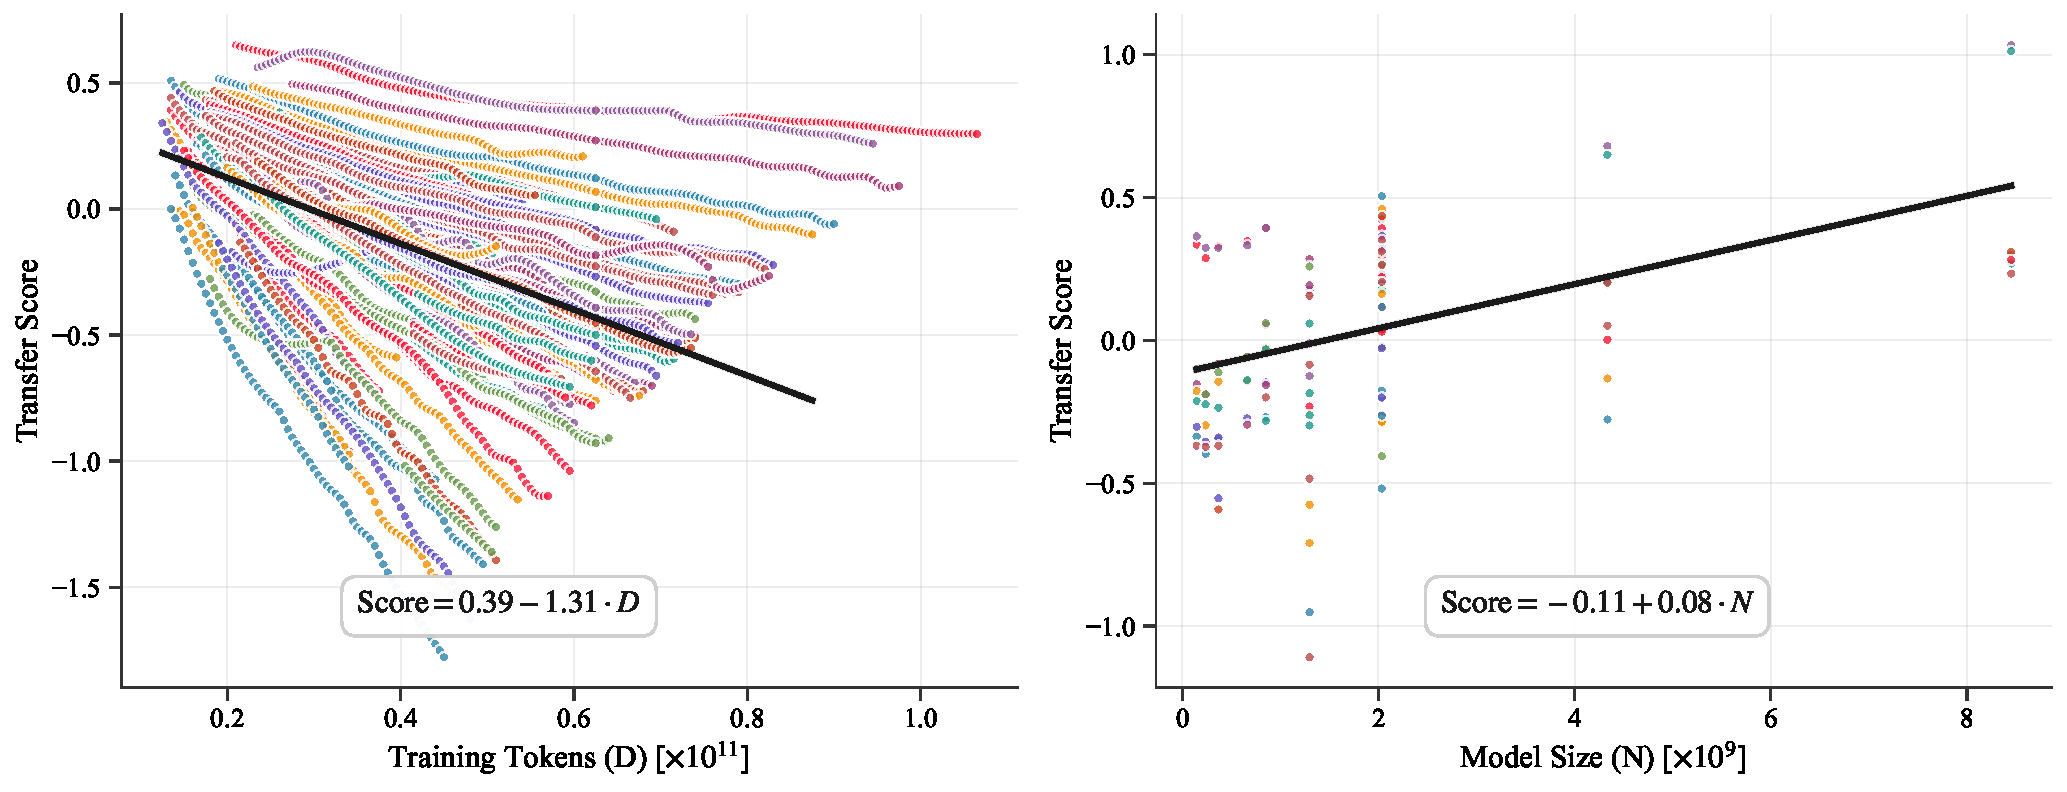
\includegraphics[width=\textwidth]{figures/language-transfer/langtransfer_dn_score_publication.pdf}
    \caption{
    \textbf{Left:} X-axis is training tokens (D), Y-axis is language-transfer score.
    \textbf{Right:} X-axis is model size (N), Y-axis is language-transfer score.}
    \label{fig:language-transfer-nd}
    \vspace{-4mm}
% \begin{figure*}[t]
%   \centering
%   %----------------------- Left panel ----------------------
%   \begin{subfigure}[t]{.5\textwidth}
%     \includegraphics[width=\linewidth]{figures/language-transfer/langtransfer_d_score.pdf}
%     \caption{X-axis is training tokens (D), Y-axis is language-transfer score.}
%     \label{fig:language-transfer-d}
%   \end{subfigure}%
%   % ← the percent sign above kills the inter-box whitespace
%   %---------------------- Right panel ----------------------
%   \begin{subfigure}[t]{.5\textwidth}
%     \includegraphics[width=\linewidth]{figures/language-transfer/langtransfer_n_score.pdf}
%     \caption{X-axis is model size (N), Y-axis is language-transfer score.}
%     \label{fig:language-transfer-n}
%   \end{subfigure}

  % \caption{\TODO{FIX FIGURE: (0) Remove titles. Add better x- and y-axis labels, and increase the font size of the ticks and labels so they are more visible. Make each figure larger, and position them so when they are side-by-side there is less whitespace between them (a tighter display). (1) Add lines connecting relevant points in the rightside figure, like in the leftside one (maybe, see how it looks). (2) Get better lines of best fit and have them annotated in a box, so we know the formula and gradient of each just by looking at the figure. (3) I don't think I like the style of having each figure in a black box. Let's just have the x and y axis visible.} \niklas{Similar to heatmap, maybe worth pointing to explanation of the transfer score so readers can reason more easily about what y=0.5 means} \sneha{nice - could we have a legend for this so we can improve the story in the text}}
\end{figure*}


\begin{figure*}
    \centering
    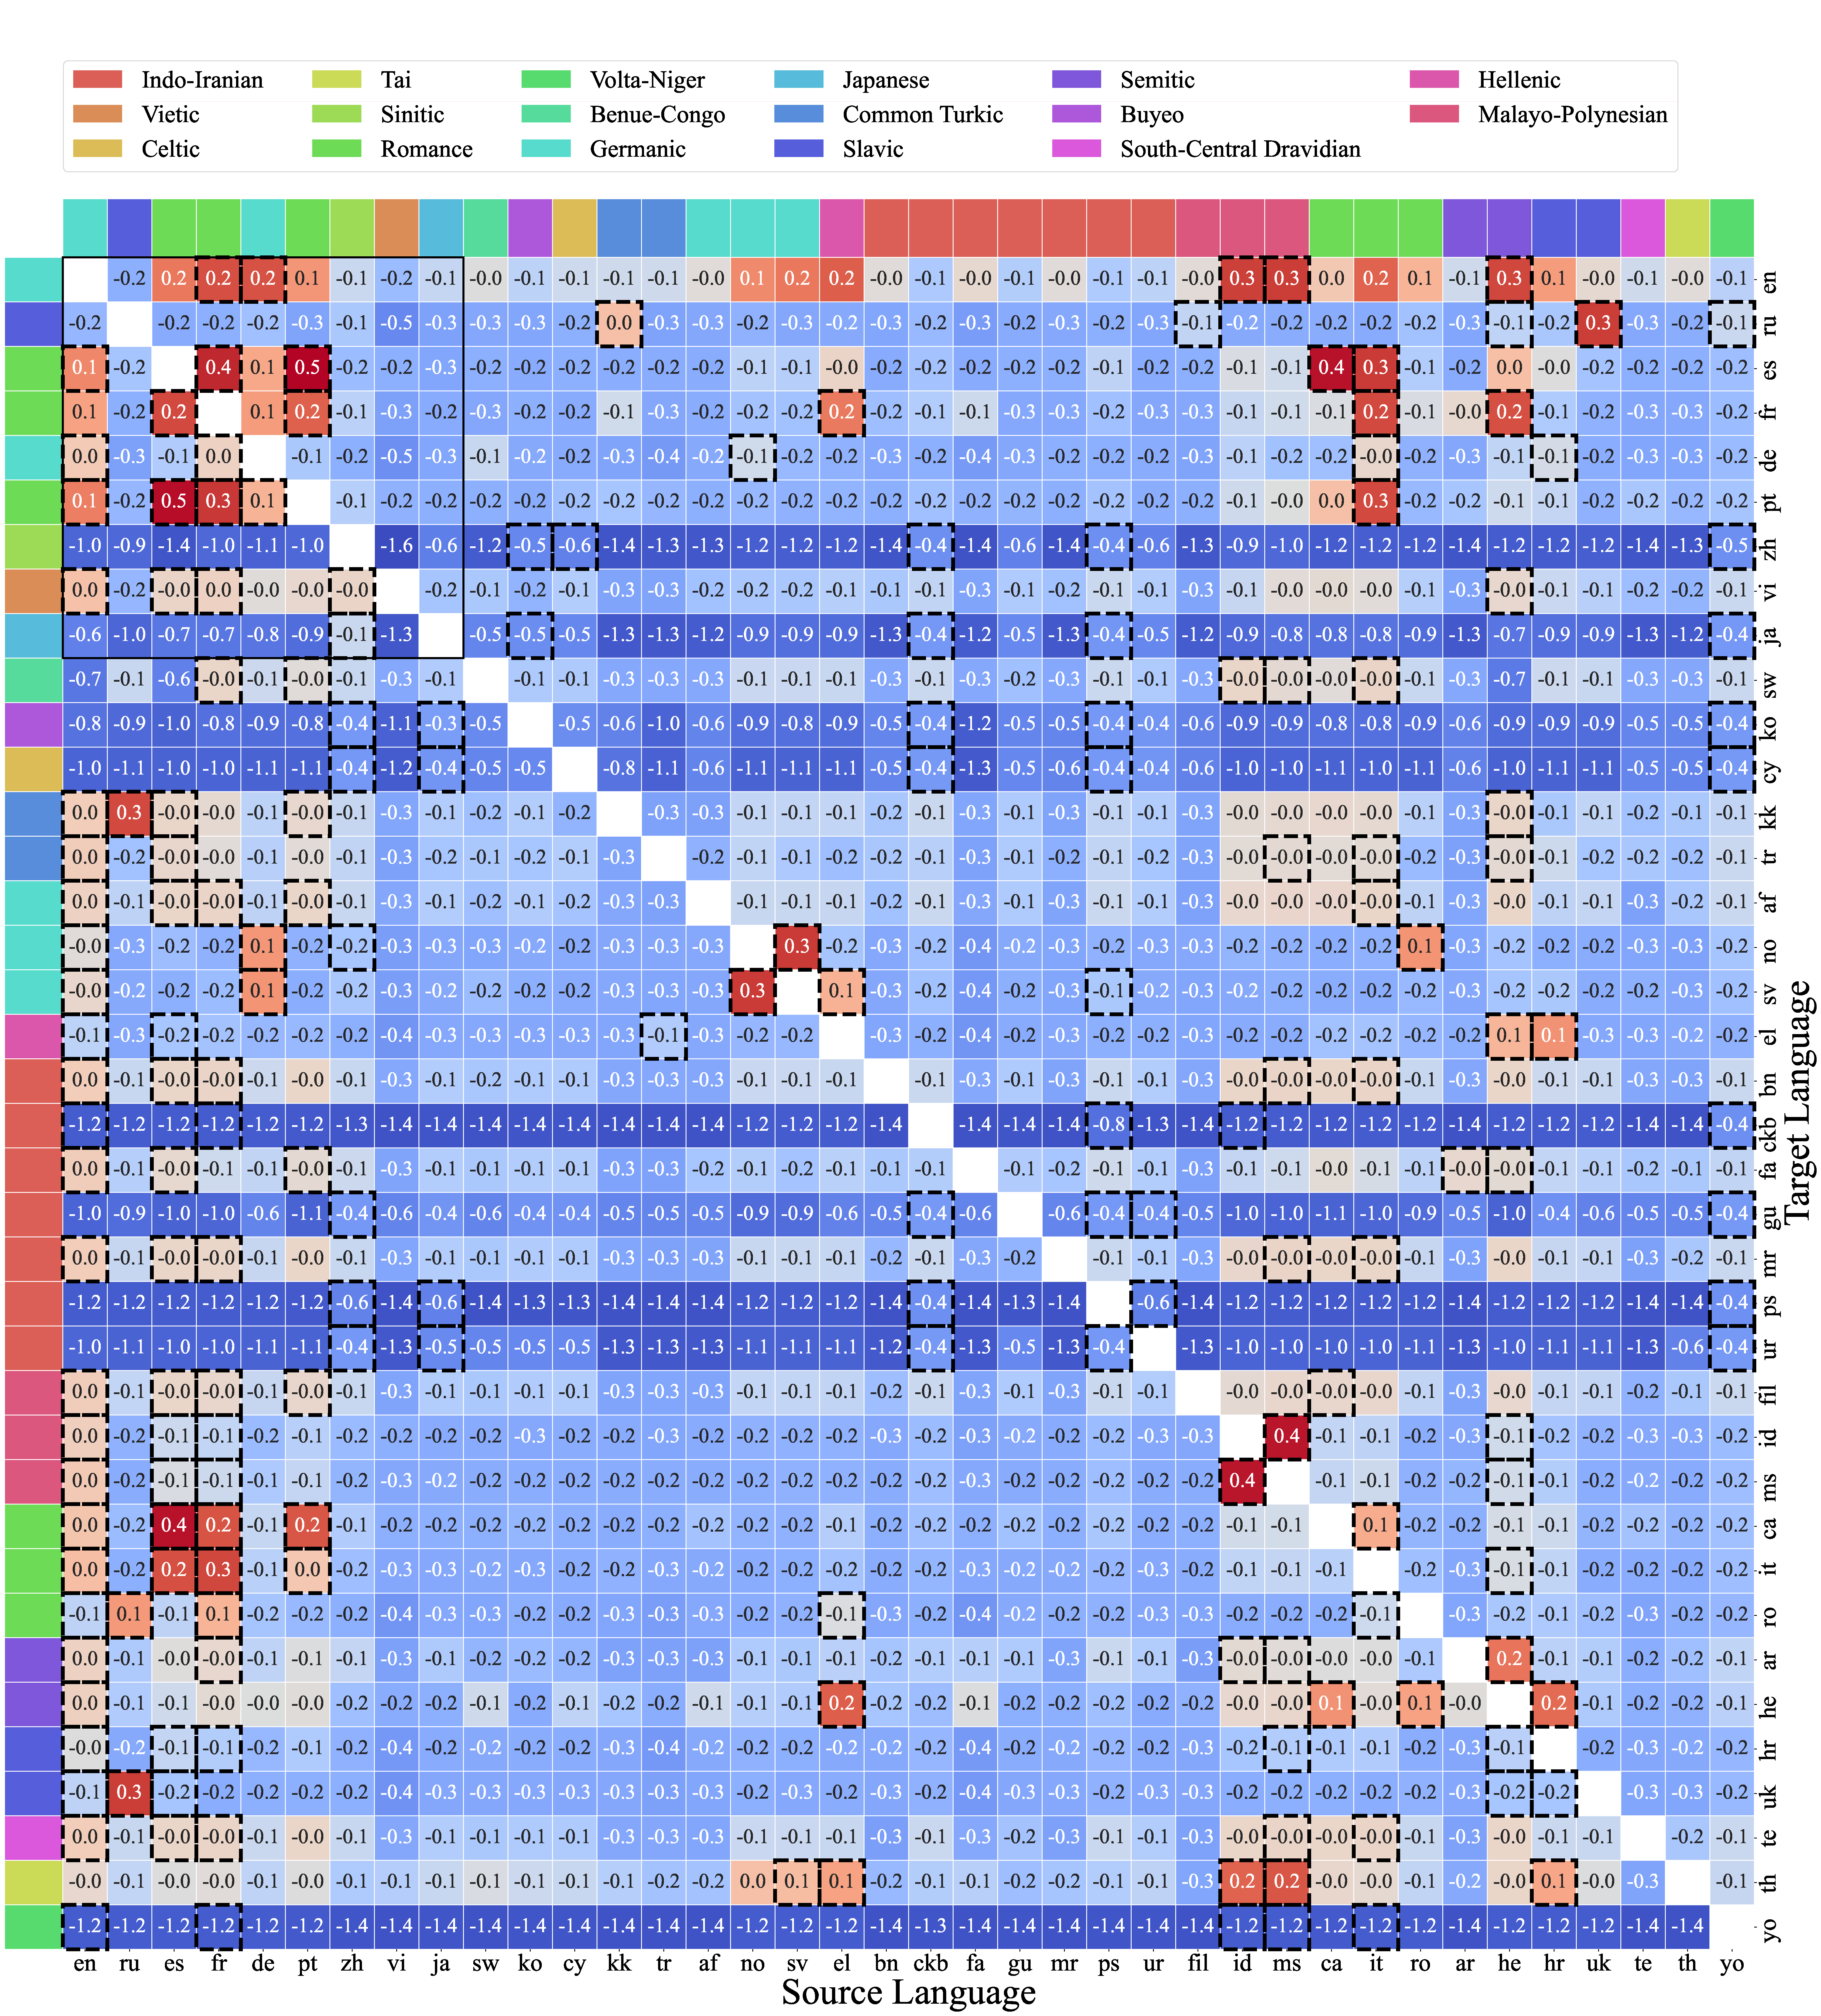
\includegraphics[width=0.9\textwidth]{figures/language-transfer/multilingual_heatmap_v1.pdf}
    \caption{The language transfer scores measure the benefit to the target language of (co-)training with the source language. We bold the top-5 source languages for each target language. The top left 9x9 are the Bilingual Transfer Score computed directly, whereas the rest are estimated from the Finetuning Adaptation Score. While English is the best source language for many of  of languages, we find language similarity is highly predictive of these scores.  \label{fig:language-transfer-heatmap-full}}
\end{figure*}





% \section{alt}

% Niklas example formulation:

% Say $D_{B \rightarrow A}$ is how much language B is worth in A terms and vice verca for $D_{A \rightarrow B}$. Consider $L_{AB}$ to be a similarity score between some language $A$ and $B$ from 0 (equal) to >>0 (very different). If we have this score and assume that it correlates directly with how useful language B is for A and vice-verca, then the problem can be broken down into:

% a) Finding the right decay function (could be exponential like in DCSL, could be linear, could be quadratic, etc), likely with a thresholding parameter $L^*$ that is learned 

% b) Deciding the range for $L_{AB}$: it could be $[0,1]$, or $[0,\infty]$,

% c) Deciding the range for $D_{B \rightarrow A}$: e.g. $[-\infty,D_A]$ (other language can harm A but never help beyond $D_A$), $[-\infty,\infty]$ (other language can harm and help even beyond $D_A$), $[0,D_A]$ (other languages can at most be neutral, help up to $D_A$)


% All of these should likely be found empirically by just codifying it and comparing $R^2$. 

% One example:

% a) exponential

% b) $[0,\infty]$

% c) $[0, D_A]$

% $D_{B \rightarrow A}=D_{B}*e^{-L^*L_{AB}}$

% here if our similarity value is 0 ($L_{AB}=0$), it is exactly one i.e. we get the full value of $D_{B}$; if the value is very high and much larger than $L^*$, then we end up with $D_{B \rightarrow A} \approx 0$.

% One thing to note is also that $L_{AB}$ may not be symmetric i.e. different from $L_{BA}$

% The full loss formula is then just
% \begin{equation}
% \label{eq:ccbase}
% L(N,D) = \frac{A}{N^\alpha} + \frac{B}{(D+D_{B \rightarrow A} + D_{C \rightarrow A} + D_{D \rightarrow A} ...) ^\beta} + E
% \end{equation}

% i.e. it is essentially the same as Chinchilla. To add multiple epochs we can then just use DCSL or any other Chinchilla extension on top of it, e.g.:

% \begin{equation}\label{eq:fin}
% \begin{aligned}
% L(U_N,U_D,R_N,R_D)=\frac{A}{(U_N + U_N R_N^* (1 - e^{\frac{-R_N}{R_N^*}}))^\alpha} + \\ \frac{B}{((U_D + U_D R_D^* (1 - e^{\frac{-R_D}{R_D^*}})) + (U_{D_{A \rightarrow B}} + U_{D_{A \rightarrow B}} R_D^* (1 - e^{\frac{-R_D}{R_D^*}}))...)^\beta} + E
% \end{aligned}
% \end{equation}

% reusing the same $R_D^*$ etc


% --- in preamble (or before the equation on the slide) ---
% \usepackage{xcolor}


% % --- on the slide ---
% \begin{align}
% \mathcal{D}_{\mathrm{eff}}^{(\text{TH})}
%   &= 
%    \underbrace{
%      \mathcal{S}_{\learned{\lambda_{\text{TH}}}}
%        \!\left(\given{D_{\text{TH}}};\,\given{U_{\text{TH}}}\right)
%    }_{\text{Thai}}
%    \\
%   &\quad+
%    \underbrace{
%      \learned{\tau_{\text{EN}}}\,
%      \mathcal{S}_{\learned{\lambda_{\text{EN}}}}
%        \!\left(\given{D_{\text{EN}}};\,\given{U_{\text{EN}}}\right)
%    }_{\text{English}}
%    +
%    \underbrace{
%      \learned{\tau_{\text{ID}}}\,
%      \mathcal{S}_{\learned{\lambda_{\text{ID}}}}
%        \!\left(\given{D_{\text{ID}}};\,\given{U_{\text{ID}}}\right)
%    }_{\text{Indonesian}}
%    \\
%   &\quad+
%    \underbrace{
%      \learned{\tau_{\text{MS}}}\,
%      \mathcal{S}_{\learned{\lambda_{\text{MS}}}}
%        \!\left(\given{D_{\text{MS}}};\,\given{U_{\text{MS}}}\right)
%    }_{\text{Malay}}
%    +
%    \underbrace{
%      \learned{\tau_{\text{HR}}}\,
%      \mathcal{S}_{\learned{\lambda_{\text{HR}}}}
%        \!\left(\given{D_{\text{HR}}};\,\given{U_{\text{HR}}}\right)
%    }_{\text{Croatian}}
%    \\
%   &\quad+
%    \underbrace{
%      \learned{\tau_{\text{ES}}}\,
%      \mathcal{S}_{\learned{\lambda_{\text{ES}}}}
%        \!\left(\given{D_{\text{ES}}};\,\given{U_{\text{ES}}}\right)
%    }_{\text{Spanish}}
%    \\
%   &\quad+
%    \underbrace{
%      \learned{\tau_{\mathrm{other}}}\,
%      \mathcal{S}_{\learned{\lambda_{\mathrm{other}}}}
%        \!\left(\given{D_{\mathrm{other}}};\,\given{U_{\mathrm{other}}}\right)
%    }_{\text{100s of other languages}} .
% \end{align}

% \medskip
% \textcolor{blue}{\textbf{Given data:}}
% $\given{D_{\ast}}$ (total tokens per language),
% $\given{U_{\ast}}$ (unique tokens / epochs).
% \quad
% \textcolor{red}{\textbf{Learned parameters:}}
% $\learned{\lambda_{\ast}}$ (repetition scales),
% $\learned{\tau_{\ast}}$ (transfer weights).

